\documentclass[letterpaper,12pt]{article}

\usepackage{threeparttable}
\usepackage{geometry}
\geometry{letterpaper,tmargin=1in,bmargin=1in,lmargin=1.25in,rmargin=1.25in}
\usepackage[format=hang,font=normalsize,labelfont=bf]{caption}
\usepackage{amsmath}
\usepackage{multirow}
\usepackage{array}
\usepackage{delarray}
\usepackage{amssymb}
\usepackage{amsthm}
\usepackage{lscape}
\usepackage{natbib}
\usepackage{setspace}
\usepackage{float,color}
\usepackage[pdftex]{graphicx}
\usepackage{listings}
\lstset{basicstyle=\footnotesize\ttfamily, language=Python, showstringspaces=false}
\usepackage{pdfsync}
\usepackage{verbatim}
\usepackage{placeins}
\usepackage{geometry}
\usepackage{pdflscape}
\synctex=1
\usepackage{hyperref}
\hypersetup{colorlinks,linkcolor=red,urlcolor=blue,citecolor=red}
\usepackage{bm}


\theoremstyle{definition}
\newtheorem{theorem}{Theorem}
\newtheorem{acknowledgement}[theorem]{Acknowledgement}
\newtheorem{algorithm}[theorem]{Algorithm}
\newtheorem{axiom}[theorem]{Axiom}
\newtheorem{case}[theorem]{Case}
\newtheorem{claim}[theorem]{Claim}
\newtheorem{conclusion}[theorem]{Conclusion}
\newtheorem{condition}[theorem]{Condition}
\newtheorem{conjecture}[theorem]{Conjecture}
\newtheorem{corollary}[theorem]{Corollary}
\newtheorem{criterion}[theorem]{Criterion}
\newtheorem{definition}{Definition} % Number definitions on their own
\newtheorem{derivation}{Derivation} % Number derivations on their own
\newtheorem{example}[theorem]{Example}
\newtheorem{exercise}[theorem]{Exercise}
\newtheorem{lemma}[theorem]{Lemma}
\newtheorem{notation}[theorem]{Notation}
\newtheorem{problem}[theorem]{Problem}
\newtheorem{proposition}{Proposition} % Number propositions on their own
\newtheorem{remark}[theorem]{Remark}
\newtheorem{solution}[theorem]{Solution}
\newtheorem{summary}[theorem]{Summary}
\bibliographystyle{aer}
\newcommand\ve{\varepsilon}
%\renewcommand\theenumi{\roman{enumi}}
\newcommand\norm[1]{\left\lVert#1\right\rVert}

\begin{document}

\title{Calibration notes for Endogenous Labor OG Model}
\date{\today}
\author{Richard W. Evans and Jason DeBacker}
\maketitle

\pagenumbering{arabic}


\section{Two methods (but really just one)}

  There are two methods to calibrate the $\chi^n_s$ parameters of the OG model with endogenous labor. The first is to use the $S$ initial-period labor supply Euler equations. The second is to use GMM to match average labor supply moments from the model steady-state to average labor supply moments from the data. The first method is orders of magnitude more simple, more intuitive, and more tractable.


  \subsection{Initial period labor supply Euler equations}

    In the model from Chapter 7 of the textbook, the general form of the labor supply Euler equation is the following.
    \begin{equation}\label{EqHHeuler_ns}
      w_t\left(c_{s,t}\right)^{-\sigma} = \chi^n_s\left(\frac{b}{\tilde{l}}\right)\left(\frac{n_{s,t}}{\tilde{l}}\right)^{\upsilon-1}\Biggl[1 - \left(\frac{n_{s,t}}{\tilde{l}}\right)^\upsilon\Biggr]^{\frac{1-\upsilon}{\upsilon}} \quad\forall s, t
    \end{equation}
    We have already estimated the elliptic utility parameter values of $b$ and $\upsilon$, and we have calibrated the value for $\sigma$ from other studies.

    All the consumption $c_{s,t}$ and wage $w_t$ values in the set of equations represented by \eqref{EqHHeuler_ns} are given in consumption units (consumption is the numeraire good). So $w_t$ represents the units of consumption that a worker is paid for each unit of labor supplied. And the implicit price of one unit of consumption is one consumption unit. This can be seen from the budget constraint.
    \begin{equation}\label{EqHHbc}
      c_{s,t} + b_{s+1,t+1} = (1 + r_t)b_{s,t} + w_t n_{s,t}
    \end{equation}
    For this reason, $c_{s,t}$ also represents the total individual consumption expenditure of age-$s$ household at in period $t$.

    One may identify the $\chi^{n}_{s}$ via a method of moments estimation that uses Equation \ref{EqHHeuler_ns} as the set of moment conditions and data on consumption, wages, and labor supply.  However, the estimates of $\chi^{n}_{s}$ will depend upon the units of measurement for wages and consumption.  Thus we could only identify the $\chi^{n}_{s}$ from the model up to a scale.  This is clearly seen if we rearrange Equation \ref{EqHHeuler_ns} to isolate $\chi^{n}_{s}$ on the left hand side:

    \begin{equation}\label{EqChi_ns}
      \chi^n_s = \frac{w_t\left(c_{s,t}\right)^{-\sigma}}{\left(\frac{b}{\tilde{l}}\right)\left(\frac{n_{s,t}}{\tilde{l}}\right)^{\upsilon-1}\Biggl[1 - \left(\frac{n_{s,t}}{\tilde{l}}\right)^\upsilon\Biggr]^{\frac{1-\upsilon}{\upsilon}}} \quad\forall s, t
    \end{equation}


  \subsection{Scaling}

    We have assumed that $\tilde{l}=1$. Regardless of the value, the appearance of $\frac{n_{s,t}}{\tilde{l}}$ denominator on the right-hand-side of \eqref{EqChi_ns} is a unit-free percent of total time endowment. However, both consumption $c_{s,t}$ and wages $w_t$ on the right-hand-side of \eqref{EqChi_ns} are in model units (consumption units).

    To overcome this identification issue, consider a scaling that relates model units to data units.  Call this parameter $factor_t$ and define it as:

    \begin{equation}\label{EqDataModelIncome}
      factor_t = \frac{\bar{y}^{data}_t}{\bar{y}^{model}_t} \quad\forall t \ \implies \bar{y}^{data}_t = \bar{y}^{model}_t \times factor_t
    \end{equation}

    In other words, $factor$ scales model units to data units for those variables measured in consumption units in the model and nominal amounts in the data.  Thus we also have the relations

    \begin{equation}
      \begin{split}
        & w^{model}_{t} \times factor_{t} = w^{data}_{t} \\
        & c^{model}_{s,t} \times factor_{t} = c^{data}_{s,t}
      \end{split}
    \end{equation}

    With this, we can return to Equation \ref{EqChi_ns}.  Let's write two versions of this equation.  One that identifies the $\chi^{n}_{s}$ in the model and one that identifies it's data counterpart.  To be clear, let $\chi^{n}_{s}$ be the model version and $\hat{\chi}^{n}_{s}$ represent the $\chi^{n}_{s}$ to be identified from the data.  Thus we have:

    \begin{equation}\label{EqChi_ns_model}
      \chi^n_s = \frac{w^{model}_t\left(c^{model}_{s,t}\right)^{-\sigma}}{\left(\frac{b}{\tilde{l}}\right)\left(\frac{n_{s,t}}{\tilde{l}}\right)^{\upsilon-1}\Biggl[1 - \left(\frac{n_{s,t}}{\tilde{l}}\right)^\upsilon\Biggr]^{\frac{1-\upsilon}{\upsilon}}} \quad\forall s, t
    \end{equation}

    and

    \begin{equation}\label{EqChi_ns_data}
      \hat{\chi}^n_s = \frac{w^{data}_t\left(c^{data}_{s,t}\right)^{-\sigma}}{\left(\frac{b}{\tilde{l}}\right)\left(\frac{n_{s,t}}{\tilde{l}}\right)^{\upsilon-1}\Biggl[1 - \left(\frac{n_{s,t}}{\tilde{l}}\right)^\upsilon\Biggr]^{\frac{1-\upsilon}{\upsilon}}} \quad\forall s, t \quad\text{where}\quad \hat{\chi}^n_s\equiv factor_t^{1-\sigma}\chi^n_s
    \end{equation}

    Note that for brevity, we do not have $data$ or $model$ superscripts on the labor supply terms.  This is because, as noted above, labor supply is always divided by labor endowment and so the ratio is in percentages both in the data and the model.

    Now let's do some algebra with Equation \ref{EqChi_ns_model}:

    \begin{equation}\label{EqChi_ns_model_algebra}
      \begin{split}
        \chi^n_s & = \frac{w^{model}_t\left(c^{model}_{s,t}\right)^{-\sigma}}{\left(\frac{b}{\tilde{l}}\right)\left(\frac{n_{s,t}}{\tilde{l}}\right)^{\upsilon-1}\Biggl[1 - \left(\frac{n_{s,t}}{\tilde{l}}\right)^\upsilon\Biggr]^{\frac{1-\upsilon}{\upsilon}}} \quad\forall s, t \\
        \implies factor^{1-\sigma}_{t} \chi^{n}_{s} & = \frac{factor^{1-\sigma}_{t}w^{model}_t\left(c^{model}_{s,t}\right)^{-\sigma}}{\left(\frac{b}{\tilde{l}}\right)\left(\frac{n_{s,t}}{\tilde{l}}\right)^{\upsilon-1}\Biggl[1 - \left(\frac{n_{s,t}}{\tilde{l}}\right)^\upsilon\Biggr]^{\frac{1-\upsilon}{\upsilon}}} \quad\forall s, t \\
        \implies factor^{1-\sigma}_{t} \chi^{n}_{s} & = \frac{\left(factor_{t}w^{model}_t\right)\left(factor_{t} c^{model}_{s,t}\right)^{-\sigma}}{\left(\frac{b}{\tilde{l}}\right)\left(\frac{n_{s,t}}{\tilde{l}}\right)^{\upsilon-1}\Biggl[1 - \left(\frac{n_{s,t}}{\tilde{l}}\right)^\upsilon\Biggr]^{\frac{1-\upsilon}{\upsilon}}} \quad\forall s, t \\
        \implies factor^{1-\sigma}_{t} \chi^{n}_{s} & = \underbrace{\frac{w^{data}_t\left( c^{data}_{s,t}\right)^{-\sigma}}{\left(\frac{b}{\tilde{l}}\right)\left(\frac{n_{s,t}}{\tilde{l}}\right)^{\upsilon-1}\Biggl[1 - \left(\frac{n_{s,t}}{\tilde{l}}\right)^\upsilon\Biggr]^{\frac{1-\upsilon}{\upsilon}}}}_{=\hat{\chi}^{n}_{s}} \quad\forall s, t \\
        \implies \hat{\chi}^n_s &\equiv factor^{1-\sigma}_{t} \chi^{n}_{s} \quad\forall s, t
      \end{split}
    \end{equation}

    Thus, by estimating $\hat{\chi}^{n}_{s}$ using the data on wages, consumption, and labor supply, one finds the model parameters up to a scale.  That scale is function of the model scale parameter, $factor_{t}$.

    \subsection{Changes to Model Solution Algorithm}
    In theory, one wants to use the factor from model period $t$, where model period $t$ corresponds to they year of your data (e.g., if the data are from 2017 and your initial period in the time path of your model is 2017, then you'd want determine the factor as $factor_{0}=\frac{\bar{y}^{data}_{2017}}{\bar{y}^{model}_{0}}$).  Because it depends on mean model income, the factor is endogenous and depends upon $\chi^{n}_{s}$.  Therefore, there is the need for some fixed point algorithm: guess a $factor$, use that to determine $\chi^{n}_{s}$, solve the model and see if mean income in the data divided by mean income in the model returns the factor you guess, if not, update and do again.  To compute the time path at each step in this fixed point algorithm would be very expensive.  We therefore make a simplifying assumption.  In particular, we assume that the factor is determined as the ratio of income in data from year $t$ and from the model's steady state.  That is,

    \begin{equation}
      factor_{t}=factor=\frac{\bar{y}^{data}_{2017}}{\bar{y}^{model}_{SS}} \ \forall t
    \end{equation}

    While not a perfect mapping, this means that at each iteration of the fixed point algorithm that solves for the model $factor$ only the steady state needs to be computed.  Also note that the model income represents real, stationarized income.  So growth and inflation are not affecting this measurement, which helps this approximation be more accurate.

    The modification to the algorithm to solve the steady state in Chapter 7 need only be modified to include the guess of $factor$ as one of our outer-loop variables along with $\bar{r}$ in the steady-state computational approach.  Given the guess for $\bar{r}$ and $factor$ one can use the relation in Equation \ref{EqChi_ns_model_algebra} to transform the $\hat{\chi}^{n}_{s}$ into the model-scaled parameter. With these $\chi^n_s$ values, we can solve for the steady-state household decisions $\{\bar{n}_s\}_{s=1}^S$ and $\{\bar{b}_s\}_{s=2}^S$. From these decisions, we can compute the corresponding steady-state interest rate $\bar{r}$ and average household income in the model $\bar{y}$. We update $\bar{r}$ and $factor$ until the interest rate and factor implied by steady state equilibrium equal the guesses of $\bar{r}$ and $factor$ at that iteration.  Once the steady state is solved and $factor$ is determined, then this same factor is applied over the time path, so no adjustment is needed for that solution method.

  \subsubsection{A Note About Initial the Initial Guess for \textit{factor}}

    Because the difference between model units and real world units might be multiple orders of magnitude, it is helpful to get the initial guess for $factor$ near its true value. If one has trouble finding an initial guess that will not break the model, a good strategy is to compute the steady-state of the model assuming that $\chi^n_s=1$ for all $s$. This means that only $\bar{r}$ is in the outer loop. Use the resulting $\bar{y}$ to derive an initial guess for $factor$ according to \eqref{EqDataModelIncome}. This should get your initial guess in the neighborhood of the final value.


\section{Data Issues}\label{SecData}

  In this section, we discuss the detail behind data issues in the calibration.


  \subsection{Consumption data}\label{SecDataCons}

    The main equation \eqref{EqChi_ns_model_algebra} requires data on consumption expenditures by age $c_{s,t}$. For the United States, we use the \href{https://www.bls.gov/cex/}{Consumer Expenditures Survey (CEX)} published by the U.S. Bureau of Labor Statistics. These data represent annual consumption expenditures by households in the survey. The survey is then used for many analyses and summaries of U.S. consumption patterns using characteristics of the underlying survey respondents and their corresponding population weights.

    In \href{https://github.com/OpenSourceMacro/LaborCalibrate/issues/5}{Issue \#5} of the \href{https://github.com/OpenSourceMacro/LaborCalibrate}{LaborCalibrate} repository, we detail two methods for calculating average consumption expenditure by arbitrary age bins.

    \begin{enumerate}
      \item The CEX has summary tables of consumption by broad age categories for each year that are precomputed (\href{https://www.bls.gov/cex/2016/combined/age.pdf}{PDF} and \href{https://www.bls.gov/cex/2016/combined/age.xlsx}{Excel}). These summary data look like the light blue bars in Figure \ref{FigCEXsummary}. One thing we could do to get consumption expenditure by arbitrary age---which is different and/or finer than the course age bins in the summary data---is to fit a curve to the summary data such that the curve has a similar shape and the average consumption expenditure across the ages corresponding to the summary data equals the value of the summary data.

      \item The more accurate thing we could do is to use the \href{https://www.bls.gov/cex/pumd.htm}{CEX survey microdata (PUMD)} itself to calculate average consumption expenditure for each age group. There is a good paper here by \citet{VillaverdeKrueger:2007}. This paper calculates exactly the lifecycle consumption profiles by age that we are interested in using the CEX microdata. For our calibration, we would probably want to average data from two or three of the most recent surveys in order to get rid of any noise that comes with the fine granularity of one-year age bins.
    \end{enumerate}

    \begin{figure}[htb]\centering\captionsetup{width=4.0in}
      \caption{\textbf{CEX consumption by age summary}}\label{FigCEXsummary}
      \fbox{\resizebox{4.0in}{3.0in}{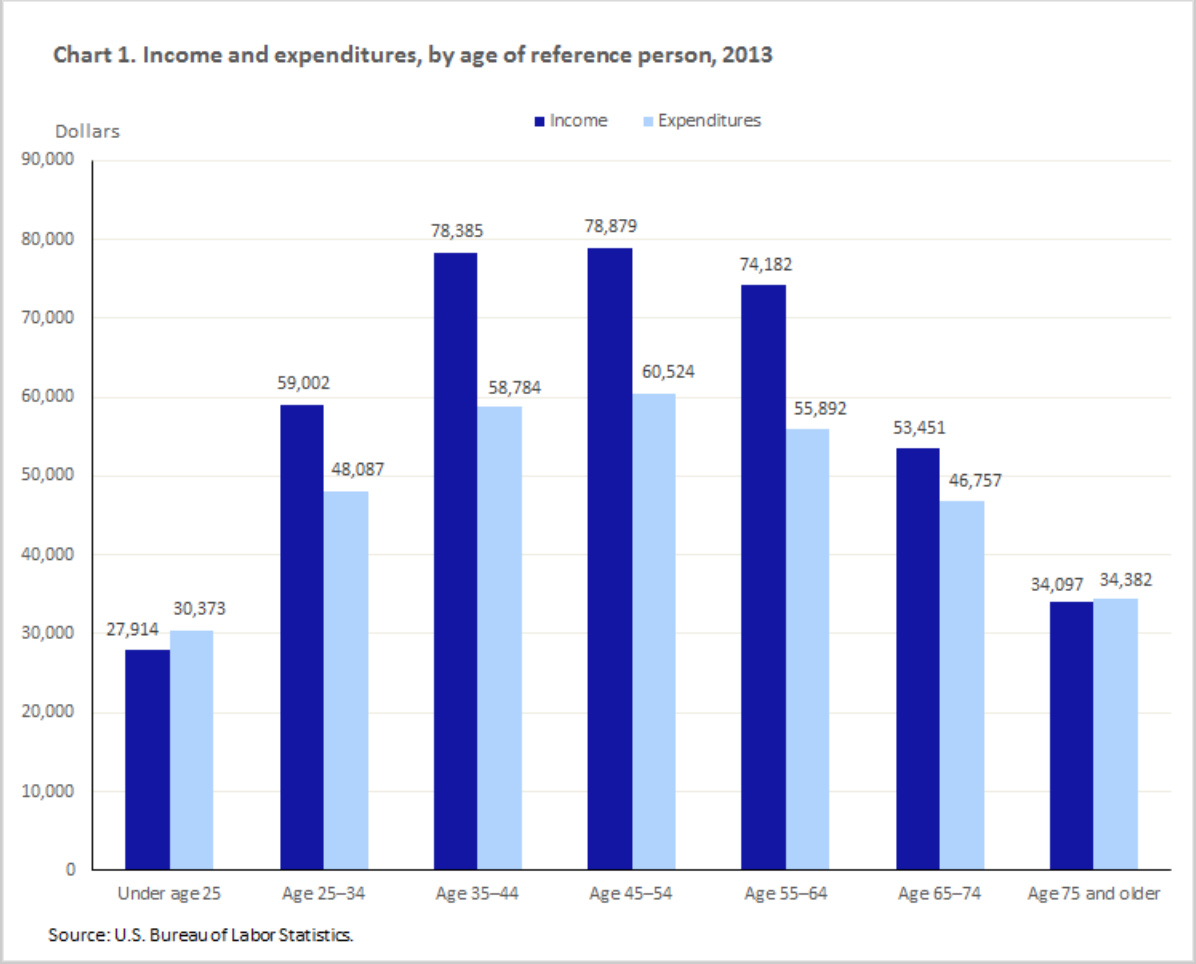
\includegraphics{images/CEXbyAgeSummary.png}}}
    \end{figure}


    \subsubsection{CEX interpolation}\label{SecDataConsInterp}

      This section details a method for following approach (1) in the previous section for using CEX summary data by age to estimate a general function for consumption by age. This approach is nice because it bypasses dealing with the individual response-level data in the CEX survey microdata (PUMD). However, it requires more technical numerical care to estimate the function properly.

      The guiding principle and assumption for this approach is that a continuous function $c(s)$ of consumption expenditure as a function of a continuous age variable $s$ exists that has the same approximate shape as the CEX summary data. Figure \ref{FigCEXsummaryGen} shows a generalization of the histogram of consumption expenditure in Figure \ref{FigCEXsummary}. If the original data have $I$ histogram bars, then the age bin cutoffis are given by the $I+1$ age values with subscripts $\{s_i\}_{i=0}^I$. An ordered age index for each of the bars as well as the average consumption expenditure for each age bin are given by $I$ respective age and consumption values with a superscript $\{s^i, c^i\}_{i=1}^I$. We have also included $I$ midpoints of each of the age bins $\{m^i\}_{i=1}^I$ as a convenient reference age within each bin. With this notation, we can say that each age bin $s^i$ is characterized by all ages between $s_{i-1}$ and $s_i$, and $c^i$ represents that average consumption of a household with a reference person with age between $s_{i-1}$ and $s_i$.

      \begin{figure}[htb]\centering\captionsetup{width=4.0in}
        \caption{\textbf{Consumption expenditure by age summary generalization}}\label{FigCEXsummaryGen}
        \fbox{\resizebox{4.0in}{2.7in}{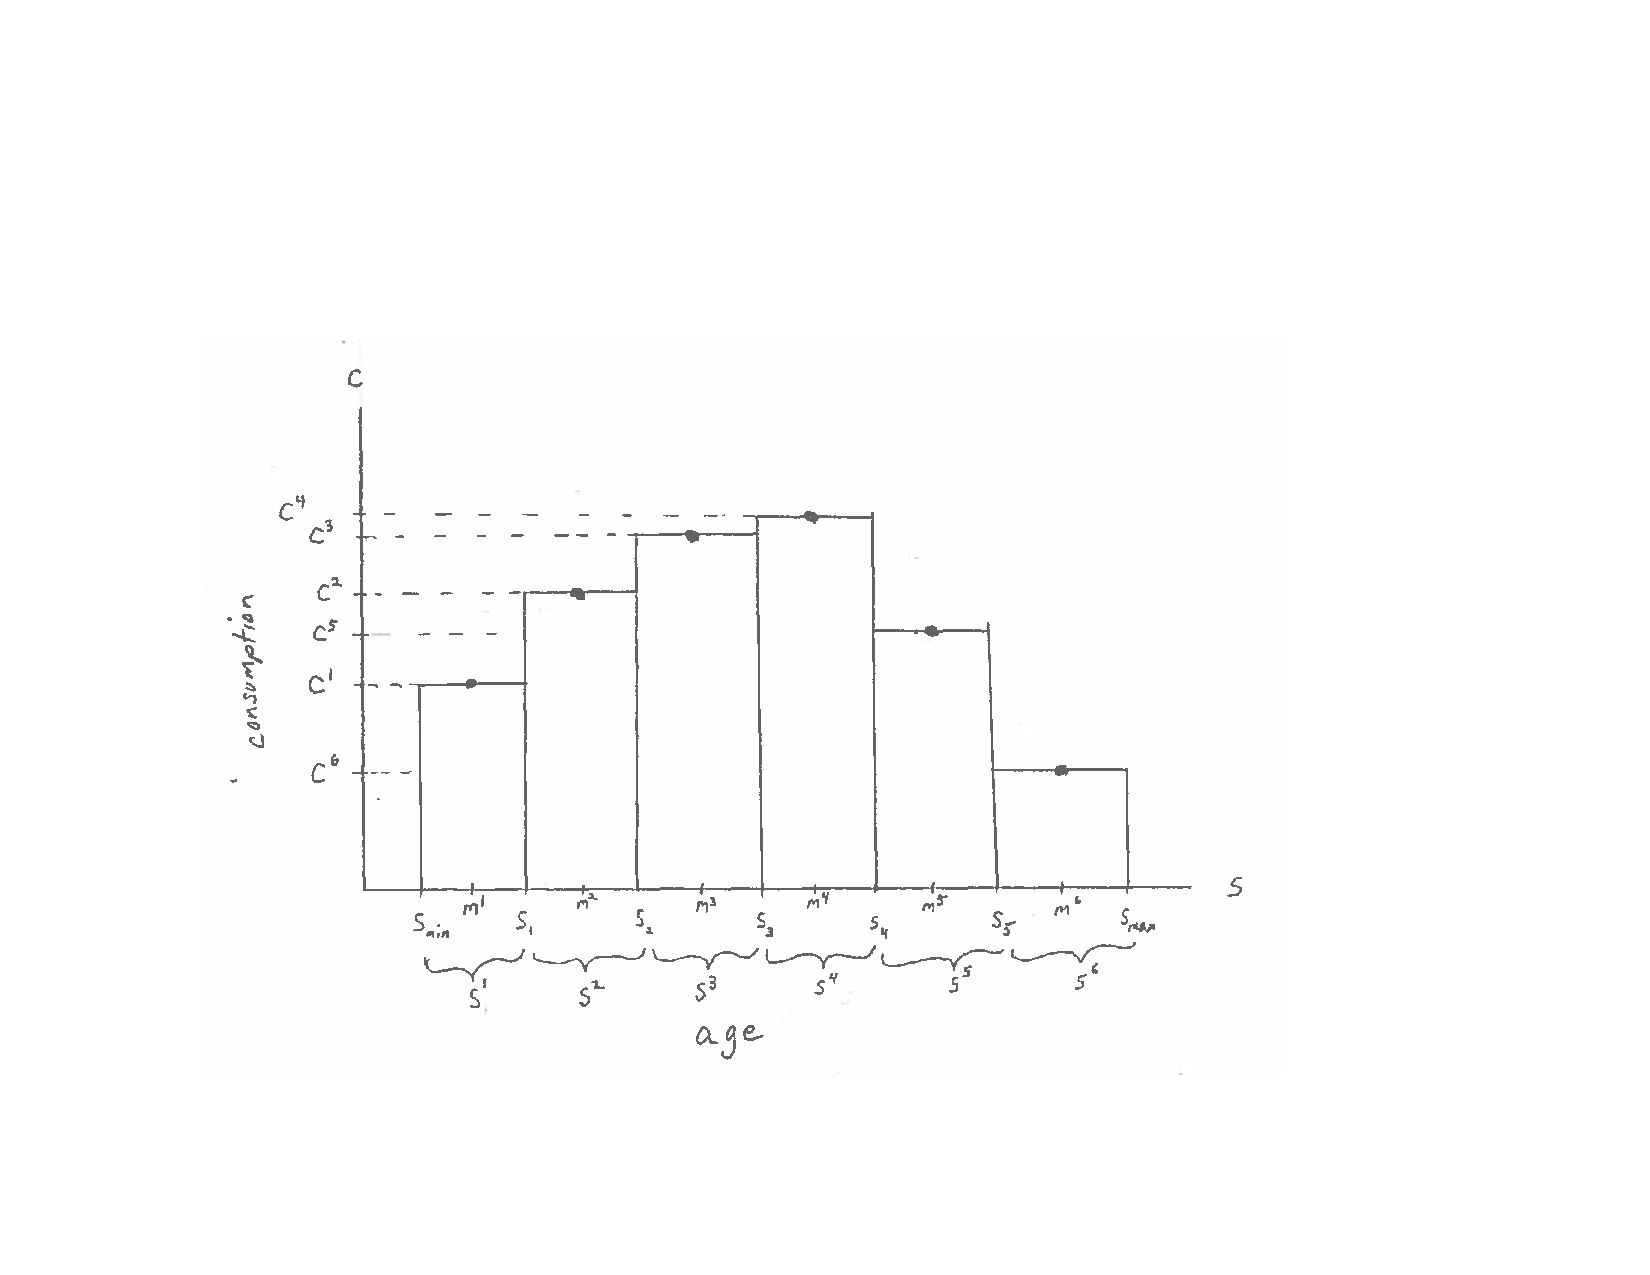
\includegraphics{images/CEXbyAgeSummaryGen.pdf}}}
      \end{figure}

      As was mentioned at the beginning of this section, the average consumption values $\{c^i\}_{i=1}^I$ in Figure \ref{FigCEXsummaryGen} are generated by an underlying continuous function of age $c(s)$. If one knows the continuous function $c(s)$ and the population density by age $f(s)$ such that $\int_s f(s)ds = 1$, one can solve for any arbitrary average consumption of an age bin $s^i$ bounded by cutoffs $s_{i-1}$ and $s_i$ using the following expression,
      \begin{equation}\label{EqCi_integral}
        c^i = \int_{s_{i-1}}^{s_i}\frac{f(s)c(s)}{F(s_i) - F(s_{i-1})}ds
      \end{equation}
      where $F(s_i)$ is the cumulative distribution function (CDF) of the continuous density function $f(s_i)$.
      \begin{equation}\label{EqCDFdef}
        F(s_i)\equiv\int_{-\infty}^{s_i}f(s)ds
      \end{equation}

      The first step toward approximating the continuous function $c(s)$ is to use the assumption that it will have roughly the same shape as the course histogram of age bins and average consumptions $\{s^i,c^i\}_{i=1}^I$. Figure \ref{FigCEXhistPointsInterp} is a scatter plot of the points $\{m^i,c^i\}_{i=1}^6$ corresponding to the light blue histogram bars in Figure \ref{FigCEXsummary}. The code for generating Figure \ref{FigCEXhistPointsInterp} is given below.

      \vspace{5mm}
      \begin{lstlisting}[frame=single]
        # Import libraries
        import numpy as np
        import scipy.interpolate as si
        import matplotlib.pyplot as plt
        from matplotlib.ticker import MultipleLocator

        # Read in (create) the data
        avg_cons = np.array([29000, 29200, 30373, 48087, 58784,
                             60524, 55892, 46757, 34382, 29000])
        age_cuts = np.array([-1, 0, 5, 25, 35, 45, 55, 65, 75, 105,
                             106])
        age_midp = np.array([-0.5, 2.5, 12.5, 30, 40, 50, 60, 70, 90,
                             105.5])

        # Generate interpolation function for consumption
        # expenditures and use to get interpolated values
        cons_func = si.interp1d(age_midp, avg_cons, kind='cubic')
        age_fine = np.linspace(-0.5, 105.5, 1000)
        cons_interp = cons_func(age_fine)

        # Solve for factor_c and c(s) function
        factor_c = 1.1 # This skipped spot is for factor_c calculation
        c_s_pts = (factor_c * (cons_interp - 29000)) + 29000

        # Create the scatter plot with interpolated curves
        fig, ax = plt.subplots()
        plt.scatter(age_midp[2:-1], avg_cons[2:-1], s=70, c='blue',
                    marker='o', label='Data')
        plt.scatter([age_midp[0], age_midp[1], age_midp[-1]],
                    [avg_cons[0], avg_cons[1], avg_cons[-1]], s=70,
                    c='red', marker='o', label='Added data')
        plt.plot(age_fine, cons_interp, c='green', linestyle='--',
                 label='Cubic spline $c_{tilde}(s)$')
        plt.plot(age_fine, c_s_pts, c='black', linestyle='-',
                 label='$c(s)$')
        minorLocator = MultipleLocator(1)
        ax.xaxis.set_minor_locator(minorLocator)
        plt.grid(b=True, which='major', color='0.65', linestyle='-')
        plt.title('Average consumption expenditure by age b +
                  '$c(s^i)$', fontsize=15)
        plt.xlabel(r'Age $s$')
        plt.ylabel(r'Consumption $c(s^i)$')
        plt.xlim((-3, 113))
        plt.ylim((25000, 1.05 * c_s_pts.max()))
        plt.legend(loc='upper right')
        plt.text(-3, 18000, 'Source: Consumer Expenditure ' +
                 'Survey (CEX), 2013 Summary Data.', fontsize=9)
        plt.tight_layout(rect=(0, 0.03, 1, 1))
      \end{lstlisting}

      \begin{figure}[htb]\centering\captionsetup{width=4.0in}
        \caption{\textbf{Histogram and midpoint coordinates of consumption summary data with interpolated function}}\label{FigCEXhistPointsInterp}
        \fbox{\resizebox{4.0in}{3.0in}{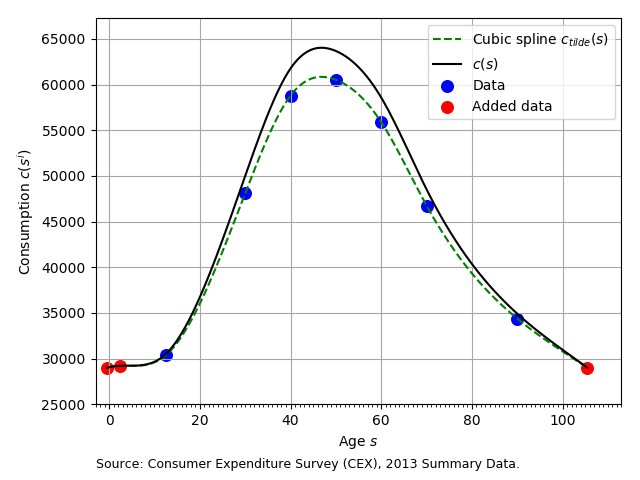
\includegraphics{images/CEXhistPointsInterp.png}}}
      \end{figure}

      Note in the \texttt{avg\_cons}, \texttt{age\_cuts}, and \texttt{age\_midp} vectors and in the two left-most point and one right-most point in Figure \ref{FigCEXhistPointsInterp}, that I added three consumption expenditure values of \$29,000, \$29,200, and \$29,000, respectively. This ensures that my interpolating function will fit the data smoothly.

      The cubic-spline interpolated function in Figure \ref{FigCEXhistPointsInterp} (green dashed line) passes through each of the scatter plot points and has continuously differentiable first and second derivatives over the support. The the cubic spline be represented by $\tilde{c}(s)$. The problem with the function $\tilde{c}(s)$ is that its average consumption values generated by plugging it in for $c(s)$ in Equation \ref{EqCi_integral} weighted by the population density $f(s)$ will not, in general, equal the actual average consumption values (scatter plot points) from the data.

      The final step for estimating $c(s)$ is to adjust the interpolated function $\tilde{c}(s)$ by a constant $factor_c$ that sets the average consumption expenditure implied by the model equal to the average consumption expenditure in the data. We define $c(s)$ as being proportional to $\tilde{c}(s)$ by the constant $factor_c$.
      \begin{equation}\label{EqCsCtildeS}
        c(s) \equiv \Bigl(factor_c \bigl[\tilde{c}(s) - 29,000\bigr]\Bigl) + 29,000
      \end{equation}
      The adding and subtracting of 29,000 in Equation \eqref{EqCsCtildeS} makes the end points in the scatter plot always stay constant. Combining \eqref{EqCsCtildeS} with \eqref{EqCi_integral} gives the equation that characterizes the constant $factor_c$.
      \begin{equation}\label{EqFactor_c}
        \text{Avg. CEX in data} = \int_{s_{min}}^{s_{max}}\frac{f(s)\biggl[\Bigl(factor_c \bigl[\tilde{c}(s) - 29,000\bigr]\Bigr) + 29,000\biggr]}{F(s_{max}) - F(s_{min})}ds
      \end{equation}
      Once $factor_c$ is estimated from \eqref{EqFactor_c}, that value with the continuous interpolated function $\tilde{c}(s)$ can be plugged in to \eqref{EqCsCtildeS} to get the estimate for the fundamental continuous consumption expenditure function that can be used to create any average consumption expenditure moments $c(s^i)$.

      The dark solid line in Figure \ref{FigCEXhistPointsInterp} shows the final $c(s)$ function.

\bibliography{CalibrationNotes.bib}


\end{document}
